\section{Results}
\label{sec:results}

\subsection{Policies}

Figure \ref{fig:controls} compares the learned controls with the analytic solution along the trajectory simulated with the learned policy. The abatement rate follows the analytic path, which rises from about 9\% in the first period to full abatement in 2175 (DICE 2016) and 2195 (DICE 2023), with a mean absolute deviation of 0.014 and 0.012 over the periods up to 2300 (Table \ref{tab:comparison}). The learned policy starts slightly low, at 6\% instead of 9\%. The largest deviations, of about 0.06, occur at the kink where the analytic rate reaches one and the constraint \(\mu \leq 1\) starts to bind; the sigmoid output of the actor rounds this kink off. The consumption rate stays within 0.013 of \(x^* = 0.7395\) in the DICE 2016 model and within 0.007 in the DICE 2023 model. The actor has learned that the optimal consumption rate does not depend on the state, although it retains small, slow drifts over time.

\begin{figure}[ht]
    \centering
    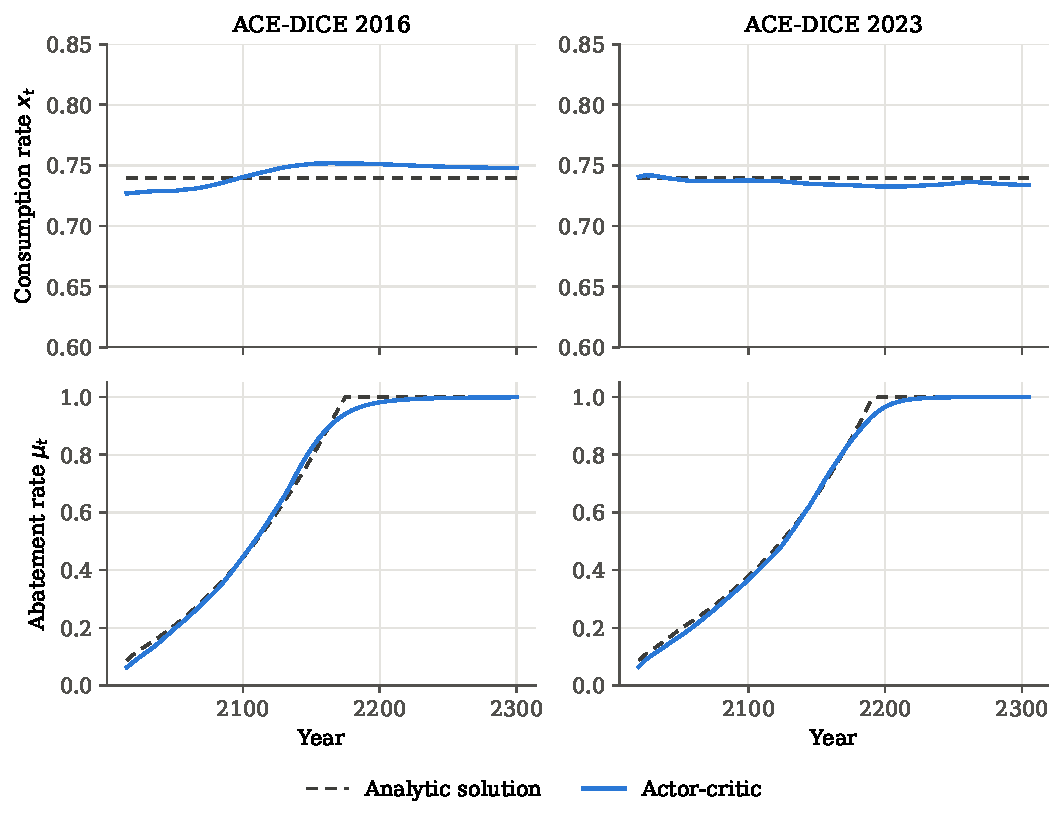
\includegraphics[width=\textwidth]{../results/figures/controls.pdf}
    \caption{Consumption rate (top) and abatement rate (bottom) of the learned policy and of the analytic solution, along the trajectory simulated with the learned policy.}
    \label{fig:controls}
\end{figure}

\begin{table}[ht]
    \centering
    \begin{adjustbox}{width=\textwidth,center}
    \begin{tabular}{lcccc}
\toprule
 & \multicolumn{2}{c}{ACE-DICE 2016} & \multicolumn{2}{c}{ACE-DICE 2023} \\
\cmidrule(lr){2-3} \cmidrule(lr){4-5}
 & Actor-critic & DEQN & Actor-critic & DEQN \\
\midrule
$\max_t |x_t - x^*|$ & 0.0126 & 0.0006 & 0.0069 & 0.0028 \\
mean $|\mu_t - \mu_t^*|$ & 0.0141 & 0.0009 & 0.0123 & 0.0020 \\
$\max_t |\mu_t - \mu_t^*|$ & 0.0582 & 0.0166 & 0.0602 & 0.0227 \\
SCC, mean relative error & 1.19\% & 0.18\% & 2.99\% & 0.56\% \\
$\lambda_k$, mean relative error & 4.88\% & -- & 2.66\% & -- \\
$\lambda_{M_1}$, mean relative error & 0.72\% & -- & 2.54\% & -- \\
$\lambda_{\tau_1}$, mean relative error & 1.42\% & -- & 1.91\% & -- \\
Welfare loss (consumption equivalent) & 0.0388\% & -- & 0.0039\% & -- \\
\bottomrule
\end{tabular}

    \end{adjustbox}
    \caption{Accuracy of the actor-critic and of a DEQN with correctly derived conditions, each against its analytic benchmark, over the periods up to 2300. Relative errors of the costates and the SCC are averaged over the same periods. The DEQN outputs costates directly, so its costate rows are reported in the companion thesis; its welfare loss is not computed.}
    \label{tab:comparison}
\end{table}

Because the learned controls are close to optimal, the simulated paths of temperature, atmospheric carbon and capital are close to the analytic optimal path (Figure \ref{fig:states}). Temperature peaks at 3.33°C in 2145 in the DICE 2016 model, as on the analytic path, and at 4.75°C in 2190 in the DICE 2023 model, against 4.72°C on the analytic path. The visible deviations after 2200 in the DICE 2023 model follow from the slower approach to full abatement around the kink.

\begin{figure}[ht]
    \centering
    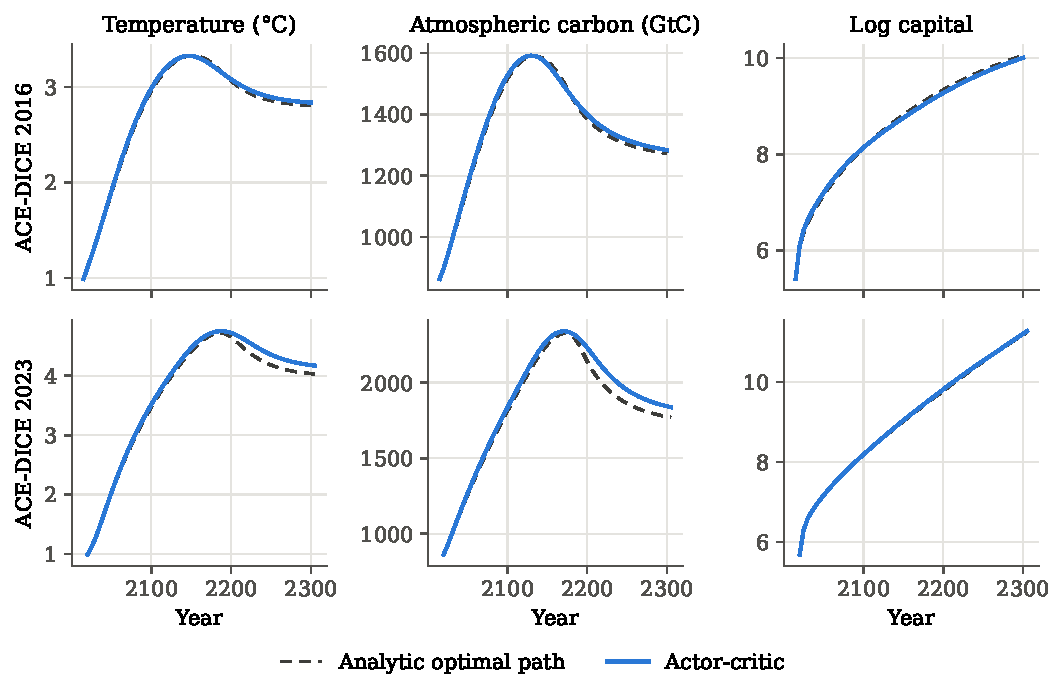
\includegraphics[width=\textwidth]{../results/figures/states.pdf}
    \caption{Temperature, atmospheric carbon and log capital under the learned policy and along the analytic optimal path from the same initial state.}
    \label{fig:states}
\end{figure}

The welfare loss of the learned policy relative to the optimum is 0.039\% of consumption in every period for the DICE 2016 model and 0.004\% for the DICE 2023 model. These losses are small because the value function is flat around the optimum: deviations in the controls cause losses in welfare that are only of second order.

\subsection{Costates and the Social Cost of Carbon}

No network in the actor-critic outputs a costate. Nevertheless, \(\beta\nabla V_\phi(\bm{s}_{t+1})\) recovers the analytic costates with mean relative errors between 0.7\% and 4.9\% (Figure \ref{fig:costates}). The carbon costate \(\lambda_{M_1} \approx -1.05 \cdot 10^{-4}\), which is four orders of magnitude smaller than the capital costate and which determines abatement, is recovered to within 0.7\% in the DICE 2016 model and 2.5\% in the DICE 2023 model. The implied SCC follows the analytic SCC closely (Figure \ref{fig:scc}), with mean relative errors of 1.2\% and 3.0\%. In 2050, the actor-critic implies an SCC of 37.0 USD/tCO\(_2\) in the DICE 2016 model and 36.9 USD/tCO\(_2\) in the DICE 2023 model, against analytic values of 37.6 USD/tCO\(_2\) in both.

\begin{figure}[ht]
    \centering
    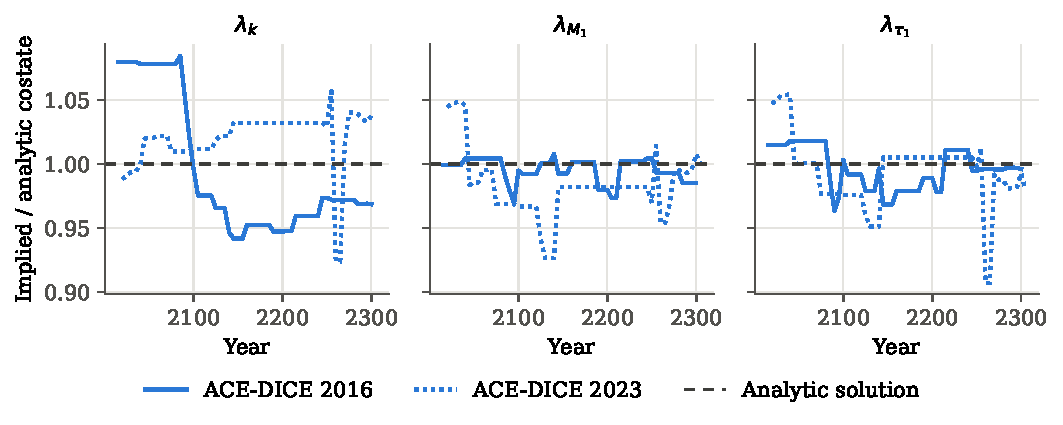
\includegraphics[width=\textwidth]{../results/figures/costates.pdf}
    \caption{Costates implied by the critic, \(\beta\nabla V_\phi(\bm{s}_{t+1})\), relative to their constant analytic values.}
    \label{fig:costates}
\end{figure}

\begin{figure}[ht]
    \centering
    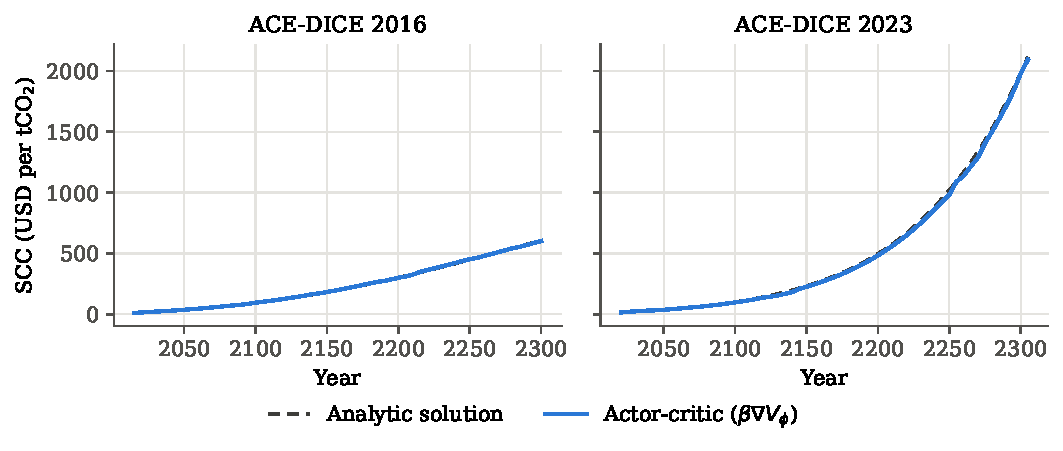
\includegraphics[width=\textwidth]{../results/figures/scc.pdf}
    \caption{SCC implied by the critic and the analytic SCC, in USD per tCO\(_2\).}
    \label{fig:scc}
\end{figure}

\subsection{Comparison with a Correctly Specified DEQN}

The DEQN with correctly derived conditions is more precise than the actor-critic, by about an order of magnitude on the controls (Table \ref{tab:comparison}). Its mean abatement error is 0.0009 and 0.0020, against 0.014 and 0.012 for the actor-critic, and its SCC errors are 0.2\% and 0.6\%, against 1.2\% and 3.0\%. This is the expected price of learning the shadow prices indirectly. The DEQN is told exactly which conditions the costates satisfy and outputs them directly, whereas the actor-critic must infer them from the curvature of a learned value function. On the other hand, the actor-critic obtains its accuracy without any hand-derived condition, so it cannot converge to the wrong solution because of a derivation error, and its gradient normalization replaces the hand-chosen scales of the DEQN. For a policy-relevant quantity such as the SCC, an error of 1--4\% is well within the uncertainty of the underlying damage and climate parameters.

\subsection{Learning Dynamics}
\label{sec:dynamics}

Figure \ref{fig:learning} shows how the errors evolve during training. During the warm-up, only the critic learns, and the implied carbon costate moves from a large, wrongly signed value towards the analytic one. At the end of the warm-up, it still has the wrong sign in both models (\(-0.14\) and \(-0.65\) times the analytic value), and the actor briefly reduces abatement. The critic corrects the sign within 25 to 50 iterations, before the actor's abatement output saturates, and abatement then rises towards its optimal path. After 1000 iterations, the implied carbon costate fluctuates between 0.84 and 1.31 times its analytic value and settles at 0.98--1.00 as the learning rate decays, while the abatement error decreases steadily to about 0.013.

\begin{figure}[ht]
    \centering
    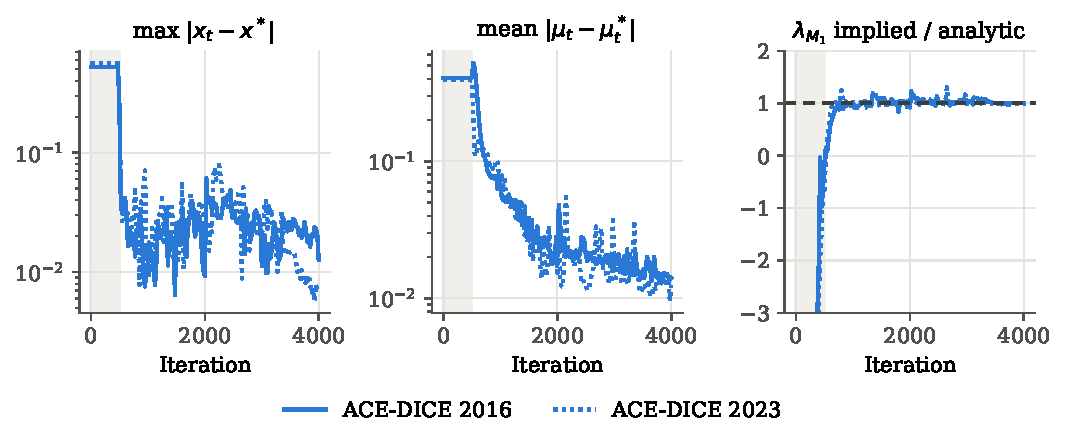
\includegraphics[width=\textwidth]{../results/figures/learning.pdf}
    \caption{Errors of the learned policy and of the implied carbon costate during training, evaluated every 25 iterations. The shaded area is the critic warm-up.}
    \label{fig:learning}
\end{figure}

\subsection{Ablations}
\label{sec:ablation}

Table \ref{tab:ablation} and Figure \ref{fig:ablation} report the two ablations for the DICE 2016 model. Both fail in the same way: the actor stops abating altogether.

\paragraph{Temporal-difference learning only.} Without the value-gradient term, the critic fits the value of its policy \emph{more} accurately than the full method, with a mean relative error of 0.02\% against the true value of the policy. Its gradient with respect to carbon, however, has the wrong sign: the implied SCC in 2050 is \(-27.7\) USD/tCO\(_2\), so that emitting carbon appears to be beneficial, and the actor sets \(\mu = 0\). The critic attributes part of the growth of the value over time, which is driven by technology and capital accumulation, to the carbon stock, which grows at the same time. This is the central lesson of the paper: an accurate value function is not sufficient for an accurate policy, because the policy depends on a gradient that is small relative to the value. The welfare loss of this policy is 0.40\% of consumption, ten times that of the full method.

\paragraph{No state perturbation.} Without perturbed states, the critic sees only the states along the trajectory, in which capital, carbon and temperature all move together. At the end of the warm-up, its carbon costate is still about \(-21\) times the analytic value, and the actor drives abatement to zero within 50 iterations. The critic does eventually learn the carbon costate, to within 2.4\% by the end of training, but by then the actor's abatement output is saturated at zero, where the gradient of the sigmoid vanishes, and the actor never recovers. The welfare loss is 0.16\% of consumption.

\begin{table}[ht]
    \centering
    \begin{adjustbox}{width=0.85\textwidth,center}
    \begin{tabular}{lccc}
\toprule
 & Full method & TD learning only & No state perturbation \\
\midrule
$\max_t |x_t - x^*|$ & 0.0126 & 0.0716 & 0.0157 \\
mean $|\mu_t - \mu_t^*|$ & 0.0141 & 0.6946 & 0.6940 \\
$\max_t |\mu_t - \mu_t^*|$ & 0.0582 & 1.0000 & 0.9997 \\
SCC, mean relative error & 1.19\% & 187.40\% & 1.82\% \\
$\lambda_k$, mean relative error & 4.88\% & 17.65\% & 5.06\% \\
$\lambda_{M_1}$, mean relative error & 0.72\% & 191.99\% & 2.45\% \\
$\lambda_{\tau_1}$, mean relative error & 1.42\% & 197.45\% & 1.18\% \\
Welfare loss (consumption equivalent) & 0.0388\% & 0.4007\% & 0.1623\% \\
\bottomrule
\end{tabular}

    \end{adjustbox}
    \caption{Ablations for the DICE 2016 model. Errors are measured as in Table \ref{tab:comparison}.}
    \label{tab:ablation}
\end{table}

\begin{figure}[ht]
    \centering
    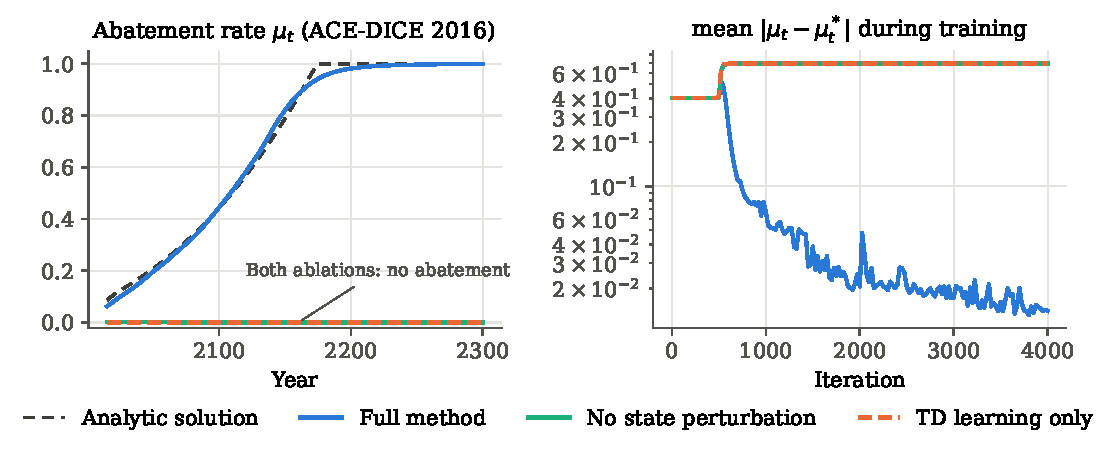
\includegraphics[width=\textwidth]{../results/figures/ablation.pdf}
    \caption{Abatement rate after training (left) and abatement error during training (right) for the full method and the two ablations, DICE 2016. Both ablations converge to zero abatement, so their lines overlap.}
    \label{fig:ablation}
\end{figure}

\subsection{Robustness Across Seeds}
\label{sec:seeds}

The results above are for one random seed. Table \ref{tab:seeds} reports the same metrics for three seeds per model, which differ in the initialization of both networks and in the state perturbations. All six runs recover the analytic solution. The mean abatement error lies between 0.010 and 0.016, the largest deviation of the consumption rate between 0.007 and 0.014, the mean relative error of the SCC between 1.0\% and 3.7\%, and the welfare loss between 0.004\% and 0.039\% of consumption.

The learning dynamics differ more between seeds than the outcomes. In three of the six runs, the critic's carbon costate still had the wrong sign when the actor started, and the actor briefly reduced abatement to 2--3\%. In each case, the critic corrected the sign within 100 to 300 iterations, before the actor's output saturated completely, and abatement recovered by iteration 800. The race described in Section \ref{sec:dynamics} is therefore real, but with state perturbations, the critic wins it in all six runs. Without perturbations, it took the critic more than 1500 iterations to correct the sign, and the actor did not recover.

\begin{table}[ht]
    \centering
    \begin{adjustbox}{width=\textwidth,center}
    \begin{tabular}{llcccccc}
\toprule
Version & Seed & $\max_t |x_t - x^*|$ & mean $|\mu_t - \mu_t^*|$ & $\lambda_k$ & $\lambda_{M_1}$ & SCC & Welfare loss \\
 & & & & \multicolumn{3}{c}{mean relative error} & (CE) \\
\midrule
2016 & 1 & 0.0126 & 0.0141 & 4.88\% & 0.72\% & 1.19\% & 0.0388\% \\
2016 & 2 & 0.0136 & 0.0150 & 2.02\% & 0.99\% & 1.01\% & 0.0374\% \\
2016 & 3 & 0.0089 & 0.0160 & 2.84\% & 1.73\% & 1.80\% & 0.0200\% \\
2023 & 1 & 0.0069 & 0.0123 & 2.66\% & 2.54\% & 2.99\% & 0.0039\% \\
2023 & 2 & 0.0099 & 0.0104 & 1.88\% & 1.07\% & 1.04\% & 0.0157\% \\
2023 & 3 & 0.0139 & 0.0137 & 4.99\% & 2.73\% & 3.70\% & 0.0160\% \\
\bottomrule
\end{tabular}

    \end{adjustbox}
    \caption{Accuracy of the actor-critic across random seeds. Seed 1 is the run reported in the rest of the paper.}
    \label{tab:seeds}
\end{table}
